\documentclass[journal,10pt,twocolumn]{article}
\usepackage{graphicx}
\usepackage{caption} 
\usepackage{hyperref}
\usepackage[margin=0.5in]{geometry}
\usepackage{booktabs}
\usepackage{array}
\usepackage{amsmath}   % for having text in math mode
\usepackage{mathtools}
\usepackage{enumitem}
\usepackage{atbegshi}% http://ctan.org/pkg/atbegshi
\AtBeginDocument{\AtBeginShipoutNext{\AtBeginShipoutDiscard}}
\newcommand{\myvec}[1]{\ensuremath{\begin{pmatrix}#1\end{pmatrix}}}
\let\vec\mathbf
\newcommand{\mydet}[1]{\ensuremath{\begin{vmatrix}#1\end{vmatrix}}}
\providecommand{\brak}[1]{\ensuremath{\left(#1\right)}}
\newcommand{\solution}{\noindent \textbf{Solution: }}
\let\vec\mathbf
\begin{document}
\begin{center}
\title{\textbf{Properties of Collinear}}
\date{\vspace{-5ex}} %Not to print date automatically
\maketitle
\end{center}
\setcounter{page}{1}
\section{10$^{th}$ Maths - Chapter 7}
\textbf{This is Problem-2 from Exercise 7.3.2}
\begin{enumerate}
\item In each of the following find the value of ‘k’, for which the points are collinear.

\item (7, –2), (5, 1), (3, k) \\
\item (8, 1), (k, – 4), (2, –5).\\

\item \textbf{Solution for problem : 1}

\begin{align}  
\vec{A}=\myvec{7 \\-2},
\vec{B}=\myvec{5 \\ 1},
\vec{C}=\myvec{3 \\ k}
\end{align}
\begin{align}
\vec{D} &=\brak{\vec{A}-\vec{B}} = \brak{\myvec{7 \\-2 } - \myvec{5 \\1 } } = \myvec{2 \\ -3 }\\
\vec{E} &= \brak{\vec{A}-\vec{C}} = \brak{\myvec{7 \\ -2 } - \myvec{3 \\k} } = \myvec{4 \\-2-k}
\end{align}
 If points on a line  are  collinear, rank of matrix is " 1 "then the vectors are in linearlydependent.
For $2\times2$ matrix Rank = 1 means Determinant is 0.
Through pivoting,we obtain
\begin{align}
\vec{F} &={\myvec{\vec{D}\\ \vec{E}}}
\end{align}
\begin{align}
\begin{split}
\myvec{
2 & -3
 \\
4 & -2-k 
}
\end{split}
\end{align}

\begin{align}
\label{eq:chem_balance_mat_row}
\myvec{
2 & -3
\\
4 & -2-k
}
 \xleftrightarrow[]{R_2 = R_2-2R_1}
\myvec{
2 & -3
\\
0 & -k+4
}
\end{align}
If the rank of the matrix has to be 1 , then -k+4=0.

\begin{align}
\begin{split}
 -k+4 &=0
\\
\implies k &=4 
\end{split}
\end{align}
\begin{figure}[h!]
	  \centering 
	  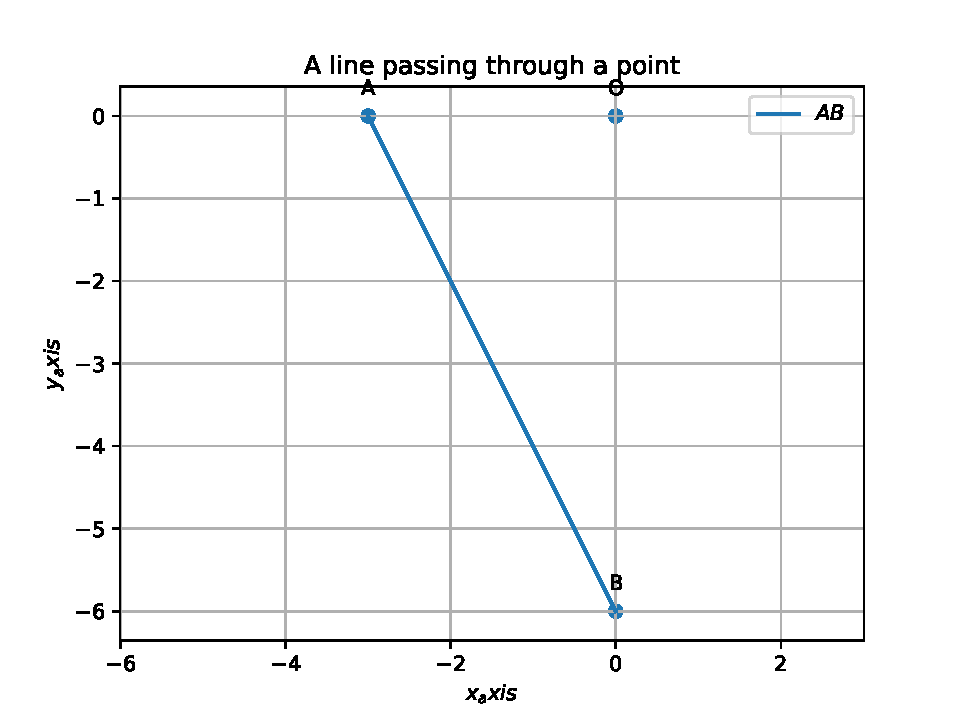
\includegraphics[width=\columnwidth]{line1.pdf}
	  \caption{}
	  \label{fig:line1.pdf}
	  \end{figure} 	 		  


 \item \textbf{Solution for problem :2}
 
\begin{align}  
\vec{A}=\myvec{8 \\ 1},
\vec{B}=\myvec{k \\ -4},
\vec{C}=\myvec{2 \\ -5}
\end{align}
\begin{align}  
 \vec{D} &=\brak{\vec{A}-\vec{B}} = \brak{\myvec{8 \\1 } - \myvec{k \\-4 } } = \myvec{8-k \\ 5 }\\
\vec{E} &= \brak{\vec{A}-\vec{C}} = \brak{\myvec{8 \\ 1 } - \myvec{2 \\-5 } } = \myvec{6 \\6}
\end{align}
If points on a line  are  collinear, rank of matrix is " 1 "then the vectors are in linearlydependent.
For $2\times2$ matrix Rank = 1 means Determinant is 0.
Through pivoting,we obtain
\begin{align}
\vec{F} &={\myvec{\vec{D}\\ \vec{E}}}
\end{align}
\begin{align}
\begin{split}
\myvec{
8-k & 5
 \\
6 & 6
}
\end{split}
\end{align}
\begin{align}
\label{eq:chem_balance_mat_row}
\myvec{
8-k & 5
\\
6 & 6
}
 \xleftrightarrow[]{R_1=\frac{R_1}{8-k}}
\myvec{
1& \frac{5}{8-k}
\\
6 & 6
}
\\
\xleftrightarrow[]{R_2 = R_2-6R_1}
\myvec{
1 & \frac{5}{8-k}
\\
\\
0 & 6-\frac{30}{8-k}
}
\end{align}
If the rank of the matrix has to be 1 , then
\begin{align}
6-\frac{30}{8-k}&=0
\end{align}
\begin{align}
 6(8-k) &= 30
\\
48-6k &= 30
\\
\implies k &=3
\end{align}
\begin{figure}[h]
	  \centering 
	  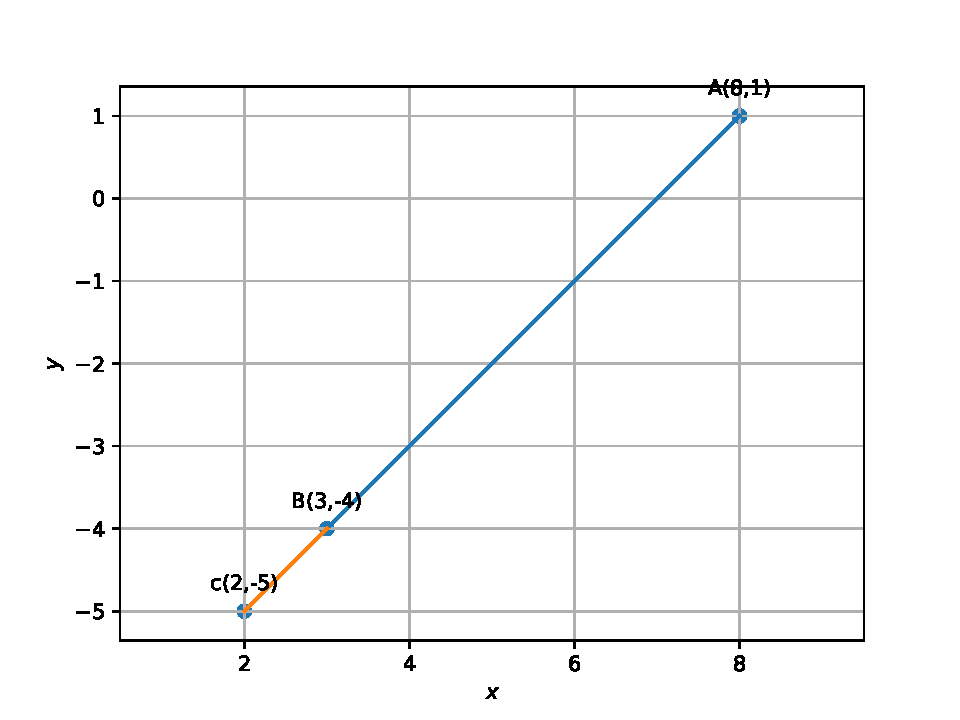
\includegraphics[width=\columnwidth]{line2.pdf}
	  \caption{}
	  \label{fig:line2.png}
	  \end{figure}
\end{enumerate} 
\end{document}
